\documentclass{article}
\pagestyle{empty}
\usepackage[utf8]{inputenc}
\usepackage[paperwidth=20cm,paperheight=3.5cm,top=0cm,bottom=0cm,left=0cm,right=0cm]{geometry}
\usepackage{tikz}
\usetikzlibrary{arrows,automata}
\usepackage{contour}
\contourlength{1pt}
\contournumber{100}

\begin{document}
\begin{center}
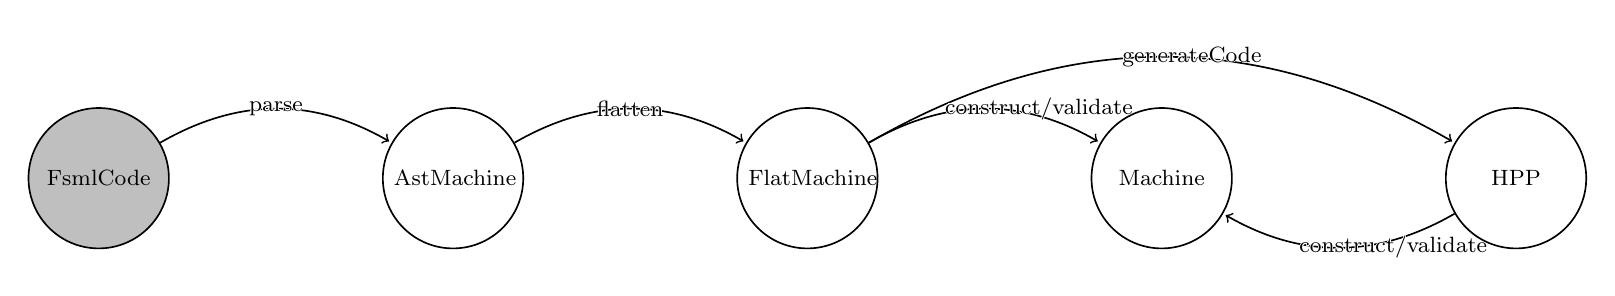
\begin{tikzpicture}[->,shorten >=1pt,node distance=4.5cm, semithick]

\tikzstyle{initial}=[fill=gray!50!white,text=black]
\tikzstyle{every node}=[font=\footnotesize]

\node[initial,state](FsmlCode){\parbox{1.5cm}{\centering FsmlCode}};
\node[state](AstMachine)[right of=FsmlCode]{\parbox{1.5cm}{\centering AstMachine}};
\node[state](FlatMachine)[right of=AstMachine]{\parbox{1.5cm}{\centering FlatMachine}};
\node[state](Machine)[right of=FlatMachine]{\parbox{1.5cm}{\centering Machine}};
\node[state](HPP)[right of=Machine]{\parbox{1.5cm}{\centering HPP}};


\path(AstMachine)edge[bend left]node{\parbox{1cm}{\centering \contour{white}{flatten} }}(FlatMachine)
(FlatMachine)edge[bend left]node{\parbox{1cm}{\centering \contour{white}{generateCode} }}(HPP)
(FlatMachine)edge[bend left]node{\parbox{1cm}{\centering \contour{white}{construct/validate} }}(Machine)
(FsmlCode)edge[bend left]node{\parbox{1cm}{\centering \contour{white}{parse} }}(AstMachine)
(HPP)edge[bend left]node{\parbox{1cm}{\centering \contour{white}{construct/validate} }}(Machine)
;

\end{tikzpicture}
\end{center}
\end{document}
